\section{Results}
\label{sec:results}

\subsection{Structured tasks show clear saturation}
\label{sec:result-structured}

Figure~\ref{fig:scaling} shows quality-versus-token curves for all six tasks.
Classification curves rise steeply at low token counts and flatten well before
level 7, with four of seven models producing F-test-significant saturating
curves ($p < 0.05$; Table~\ref{tab:ftest}).
Saturation points for these four models range from 42 to 64 tokens,
well below a typical worked-example prompt (level 7: $\approx$ 300--400 tokens).

Product extraction curves are similarly sigmoidal: three of seven models are
significant, with saturation points ranging from 92 (llama-3.3-70b) to 536
(claude-haiku) tokens.
The wider range reflects greater schema complexity: a four-field JSON extraction
requires more elaboration cues than binary sentiment labelling.
For all significant product extraction pairs, R$^2 > 0.70$, confirming strong
curve fit.

\begin{figure}[t]
  \centering
  
\includegraphics[width=\linewidth]{figures/fig_sat1_scaling_curves.png}
  \caption{Quality (LLM judge, normalised to [0,1]) vs.\ mean prompt tokens
    across seven levels, for all six tasks and seven models.
    Dashed lines show the best-fit log/sigmoid curve; dotted verticals mark the
    95\%-of-asymptote saturation point.
    Classification and product extraction show clear sigmoid curves;
    QA and math reasoning are flat.}
  \label{fig:scaling}
\end{figure}

\begin{table}[t]
\centering
\caption{F-test results and saturation points. Bold rows are significant ($p < 0.05$).
  CI: 95\% bootstrap confidence interval on saturation token count $T^*$.}
\label{tab:ftest}
\small
\begin{tabular}{llrrrr}
\toprule
Task & Model & $F$ & $p$ & $T^*$ & 95\% CI \\
\midrule
\multirow{4}{*}{Classification}
  & \textbf{gemini-flash}  & 14.5 & 0.027 & \textbf{42}  & [29, 147]  \\
  & \textbf{kimi-k2}       & 21.1 & 0.016 & \textbf{57}  & [55, 237]  \\
  & \textbf{gpt-4o-mini}   & 42.0 & 0.006 & \textbf{50}  & [46, 230]  \\
  & \textbf{llama-3.3-70b} & 22.3 & 0.015 & \textbf{64}  & [63, 72]   \\
\midrule
\multirow{3}{*}{Product Extraction}
  & \textbf{llama-3.3-70b} & 16.4 & 0.023 & \textbf{92}  & [83, 312]  \\
  & \textbf{qwen3-32b}     & 26.6 & 0.005 & \textbf{378} & [118, 506] \\
  & \textbf{claude-haiku}  & 49.6 & 0.005 & \textbf{536} & [233, 586] \\
\midrule
Summarization      & \textbf{claude-haiku}  &  9.4 & 0.031 & \textbf{83}  & [78, 87]   \\
Instr.\ Following  & \textbf{llama-3.1-8b}  & 13.1 & 0.031 & \textbf{112} & [50, 314]  \\
\midrule
QA (all 7)   & \multicolumn{4}{l}{All $p > 0.12$; not significant}      & ---        \\
Math (all 7) & \multicolumn{4}{l}{All $p > 0.70$; not significant}      & ---        \\
\bottomrule
\end{tabular}
\end{table}

\subsection{Open-ended tasks show no significant saturation}
\label{sec:result-open}

QA and math reasoning yield zero significant pairs out of seven models each.
Fitted curves have low R$^2$ (QA: 0.06--0.69; math: 0.12--0.34) and fail to
beat the flat null model at $\alpha = 0.05$ in every case.
The quality-versus-token lines appear near-horizontal in
Figure~\ref{fig:scaling}.

This is a \emph{meaningful negative result}: the same
experimental setup detects strong saturation in classification, ruling out
methodological artefact.
Two interpretations are consistent with the data:
(1) models that already score above 0.85 quality at level~1 (the bare prompt)
are near-ceiling, so additional elaboration cannot improve further;
(2) models scoring well below ceiling at level~1 are bottlenecked by
parametric knowledge or reasoning depth, neither of which is improved by
instruction tokens.

Summarization (1/7 significant, claude-haiku only) and instruction following
(1/7 significant, llama-3.1-8b only) occupy an intermediate position,
consistent with their partial schema requirements.

\subsection{Saturation points vary by task and model}
\label{sec:result-heatmap}

Figure~\ref{fig:heatmap} shows saturation token counts as a model $\times$ task
heatmap.
Within classification, points range from 42 (gemini-flash) to 64 tokens
(llama-3.3-70b) for significant pairs.
Within product extraction, the range is substantially wider (92--536 tokens),
reflecting greater schema complexity and higher variance across models.

\begin{figure}[t]
  \centering
  
\includegraphics[width=0.85\linewidth]{figures/fig_sat2_saturation_points.png}
  \caption{Saturation token counts (heatmap, model $\times$ task).
    Darker shading indicates more tokens needed for saturation.
    Cells for non-significant fits are shown in grey.}
  \label{fig:heatmap}
\end{figure}

Notably, llama-3.3-70b saturates product extraction at just 92 tokens
(CI: [83, 312]), substantially earlier than claude-haiku (536 tokens;
CI: [233, 586]).
This is consistent with capability differences: a stronger model infers the
output schema from fewer cues.

\subsection{Replication on larger dataset}
\label{sec:replication}

To verify that the observed saturation behaviour is not an artifact of the
smaller evaluation set, we replicate the experiment on a larger sample of 200
examples from standard benchmark datasets: SST-2~\citep{socher2013recursive}
for sentiment classification and SQuAD~\citep{rajpurkar2016squad} for question
answering.
The replication uses the same additive prompt levels, evaluation procedure,
and curve-fitting methodology as the main experiment.

Figure~\ref{fig:replication-curves} (Appendix~\ref{app:replication}) shows the
resulting quality--token curves.
The classification task again exhibits a clear sigmoid relationship between
prompt length and quality, with performance increasing rapidly at low token
counts and plateauing afterward.
The estimated saturation point occurs at approximately 64 tokens, consistent
with the range reported in the main experiment.

In contrast, the question answering task shows no statistically significant
relationship between prompt length and response quality.
Performance fluctuates across prompt levels without a consistent upward trend,
reinforcing the finding that open-ended tasks do not exhibit prompt saturation.

Figure~\ref{fig:replication-saturation} reports the estimated saturation token
counts, and Figure~\ref{fig:replication-ci} shows the bootstrap confidence
interval for the classification saturation point, confirming that the estimate
is stable across resampled evaluation sets.

These results confirm that the structured--open task dichotomy observed in the
main experiment persists when evaluated on a substantially larger dataset.

\subsection{Forest plot of significant saturation points}
\label{sec:result-forest}

Figure~\ref{fig:forest} plots all nine significant saturation points with
95\% bootstrap CIs.
Classification CIs are generally narrow (llama-3.3-70b: [63, 72]),
indicating precise saturation point estimation.
Product extraction CIs are wider, reflecting higher inter-example variance
in how models respond to elaboration.

\begin{figure}[t]
  \centering
  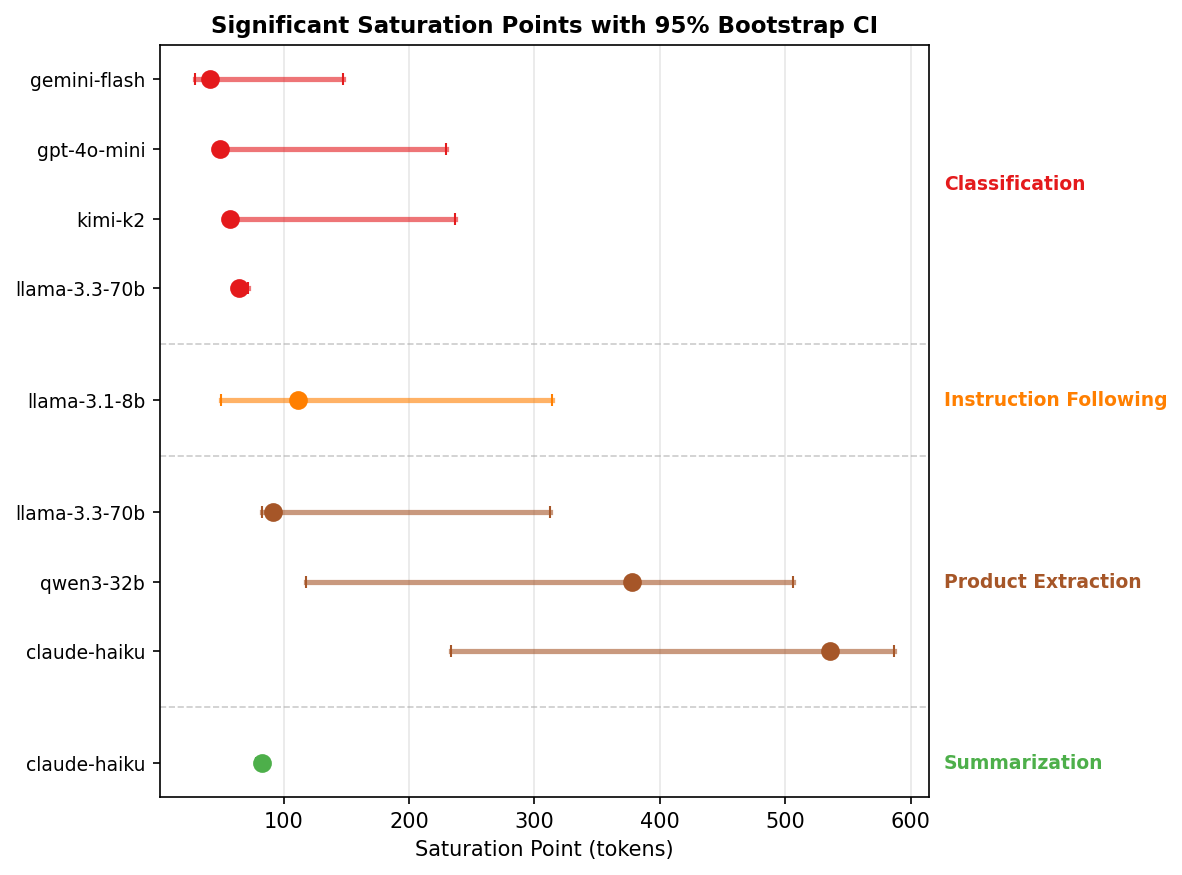
\includegraphics[width=0.82\linewidth]{figures/fig_sat3_forest_plot.png}
  \caption{Saturation points with 95\% bootstrap CIs (only F-test significant
    pairs, $p < 0.05$).
    Classification concentrates below 70 tokens (left); product extraction
    spans a wider range.}
  \label{fig:forest}
\end{figure}
